%\VignetteIndexEntry{Using icenReg}

\documentclass[a4paper]{article}
%\documentclass[11pt]{book}
\usepackage{amsmath, amsthm}
\usepackage[pdftex]{graphicx}
\usepackage{psfrag,epsf}
\usepackage{enumerate}
\usepackage{natbib}
\usepackage{float}
\restylefloat{table}

\usepackage{amssymb}
\usepackage{multirow}
\usepackage{float}


%\VignetteIndexEntry{icenReg}


\usepackage{Sweave}
\begin{document}
\Sconcordance{concordance:StatisticalBackground.tex:StatisticalBackground.Rnw:%
1 20 1 1 0 152 1 1 2 1 0 2 1 12 0 1 2 10 1 1 2 1 0 2 1 12 0 1 2 37 1 1 %
4 3 0 1 7 6 0 1 3 1 0 1 2 5 0 1 2 22 1 1 2 1 0 1 1 1 4 2 0 1 1 4 0 1 2 %
4 1 1 3 2 0 1 2 4 0 1 2 36 1 1 13 1 2 7 1 1 24 1 3 30 1}


\title{A lightning introduction to survival analysis with emphasis on interval censoring}
\author{Clifford Anderson-Bergman}
\maketitle


\tableofcontents

\section{Introduction}

\subsection{What is Survival Analysis?}

  Survival analysis is the modeling of time-to-event data. For example, a researcher may be interested in modeling the distribution of time until engine failure in a car or time until full recovery after a surgery. ``Time" can be generalized to exposure; in the engine failure example, modeling miles driven until failure may prove more precise than time until failure and would still be considered a survival analysis problem. All that is required to be a survival problem is that we have a measure such that for each subject, if the measure is below some value, the event has not occurred and if it is greater than or equal to this value, it has occurred. The term ``survival" originates from the fact that in many studies, the response of interest is time until death. 
  
  In theory, traditional statistical models (linear regression, ANOVA, etc.) can be applied to model time-to-event data. In practice, it is found that there are very frequently issues in the collected data that invalidate such models. These include \emph{censoring}, \emph{truncation} (both to be explained soon) and to a lesser extent, non-normality. As such, survival analysis tools are typically built to be robust to non-normality, censoring and (less frequently) truncation. 
  

\subsubsection{Important Functions}

  In the field of survival analysis, three new functions are commonly used to characterize a distribution. All three of these functions are a function of $f_T(t)$, the pdf/pmf of the distribution of a random variable $T$. For convience, we also define $F_T(t)$ to be the cumulative distribution function. The new functions are:
  
  \begin{itemize}
  \item Survival function: $S_T(t) = 1 - F_T(t)$
  \item Hazard function: $h_T(t) = \frac{f_T(t)}{S_T(t)}$
  \item Cumulative hazard function: 
      $H_T(t) = \displaystyle \int_{-\infty}^{t} h_T(x) dx
      =
      -\log(S_T(t))$
  \end{itemize}

  The survival function is easiest to interpret: $S_T(t)$ represents the probability of survival (if the outcome of interest is death) up to time $t$. This value is a probability, so we always have that $S(t) \in [0,1]$. Likewise, $S$ is necessarily a decreasing (but not strictly decreasing) function. Two common assumptions are that $S(0) = 1$, i.e., event times must be strictly positive, and $S(\infty) = 0$, i.e., an event will eventually happen with probability 1. 

  
  The hazard function is slightly more awkward to interpret: it is the failure rate at time $t$ conditional on survival up to time $t$. Although the hazard function is mostly motivated by the regression model built around it, in some ways the hazard function may be more relevant than the pdf/pmf for certain situations. For example, if a patient goes to a doctor to assess their risk of heart disease, they are interested in their hazard rate (given that they have not suffered heart disease), rather than the estimated pdf/pmf. The hazard function is non-negative, but not to be confused with a pdf/pmf; the integral/sum is not bounded by 1. 
  
  The cumulative hazard function does not have a nice interpretation, but proves to be mathematically convienent in many problems. It is a non-negative function. 


\subsection{What is Censoring?}

  Very frequentially, survival analysis studies exhibit censored data. This occurs when an event time for a given study is not observed exactly, but rather only known to have occurred within some range. 
  
  \subsubsection{Types of Censoring}

  \begin{itemize}
  \item Right censoring
  \end{itemize}
  
  Right censoring occurs when an event time $T$ is only known to be greater than some observed value $C$. For example, suppose a study follows subjects and records age of onset of cancer. The study ends in 10 years, and several of the subjects never developed cancer. For these subjects, we do not know the age of cancer development ($T_i$ for subject $i$), other than it is greater than the age of the subjects at the end of the study ($C_i$ for subject $i$). 

  Standard notation for right censoring is to represent the response with a tuple $\{Y_i, \delta_i\}$, with $\delta_i$ being an indicator for whether the event was observed to have occurred in the study. Formally, 
  
  \[
  \delta_i = 
  \begin{cases}
  1 & \text{if } Y_i < C_i \\
  0 & \text{if } Y_i \geq C_i\\
  \end{cases}
  \]
  
  . If $\delta_i = 1$, $Y_i$ is the observed event time for the $i^{th}$ subject (i.e., $Y_i = T_i$). If $\delta_i = 0$, $Y_i$ is the last time in which it is known the event has not occurred for the $i^{th}$ subject ($Y_i = C_i$). 

  The vast majority of the survival analysis literature focusses on right censoring. 

  \begin{itemize}
  \item Left censoring
  \end{itemize}

  Left censoring occurs when an event is only known to have occurred \emph{before} some observed value $C$. In the cancer study example, suppose a subject enrolled in the study and during the initial screening, they tested positive for cancer. In this case, the age of onset is known to be lower than the age at tested. In this case, $C$ represents the earliest time for which the event has already occurred. 
  
  Similar to right censoring, left censored data is often represented with the tuple $\{Y_i, \delta_i\}$, with $Y_i = T_i$ if $C_i \leq T_i$ (i.e. uncensored) and $Y_i = C_i$ if $C_i > T_i$  and  $\delta_i$ being an indictor for whether the $i^{th}$ subject was left censored. 

  \begin{itemize}
  \item Interval censoring
  \end{itemize}

  Interval censoring occurs when event times are only known up to an interval. In the cancer study example, suppose subjects had semi-regular doctor check ups. If a subject tested negative at one check up, but positive at the next, all that is known is that the onset occurred sometime between check ups. If these check ups are performed with high frequency (i.e., monthly check ups in this case), ignoring the interval censoring by using some simple imputation strategy will likely be inconsequential. However, if the check ups are less frequent such that using inappropriate imputation methods could significantly affect inference, interval censoring methods should be used for valid inference. 
  
  Interval censored responses are typically represented with the tuple $\{L_i, U_i\}$, where $L_i$ the lower end of the interval capturing the true event time for the $i^{th}$ subject and $U_i$ represents upper end of the interval. This allows for right censoring ($U_i = \infty$), left censoring ($L_i = 0$), general interval censoring ($0 < L_i < U_i < \infty$) and uncensored data ($L_i = U_i$). 

  A special case of interval censoring is current status data. This occurs when each subject is only inspected a single time. If the event has already occurred at the time of inspection, that subject is left censored, otherwise it is right censored. Data may be collected in this manner for cost effectiveness (no need to follow patients) or because inspection may alter the samples. As an example, sensitivity analysis for explosives involves testing new materials at different levels of impact. It is assumed that for each sample, impacts above a certain threshold will always trigger the explosive, below this threshold will never trigger the explsives, and that this threshold is random for each sample. After a failed test (i.e., failed to detonate), the sample will be damaged and is no longer suited for retesting. This results in current status data; instead of time, the exposure measurement is force of impact. If a sample failed to detonate at its tested level, it is right censored. If a sample successfully detonated, it is left censored. 

  \subsection{Censoring and the likelihood function}
  \label{sec:llk}
  We cover the case of right censoring in detail and state the results for left censoring and interval censoring. 
  
  As stated above, for each subject there exists a response time $T_i$ and a censoring time $C_i$. The tuple $\{Y_i, \delta_i\}$ is observed for each subject. Defining $f_{T, C}(t, c, \Theta)$ to be the joint pdf of $T_i$ and $C_i$, conditional on some parameters set $\Theta$, we can write the joint pdf of $\{Y_i, \delta_i\}$ 
  \footnote{Technical note: the pdf presented is under the condition that $C_i$ is unknown if the event is uncensored. In some cases, both $T_i$ and $C_i$ may be known. We will see that this distinction is inconsequential under the standard assumption of independence of $T_i$ and $C_i$.} as

  
  \[
  f_{Y_i, \delta_i}(y, \delta) = \left( \int_{-\infty}^{y} f_{T, C} (y, x, \Theta) dx \right) ^ {\delta}
  \left( \int_{y}^{\infty} f_{T, C} (x, y, \Theta) dx \right) ^{(1-\delta)}.
  \]

  In otherwords, if $Y_i$ is uncensored with value $y$, then $C_i \leq y$ and so we intergrate over this range of $C_i$ in the pdf of $\{Y_i, \delta_i\}$. If $Y_i$ is censored, then $T_i > y$, and we integrate over this range of $T_i$ in the pdf. 
  
  In order to make this problem more tractable, it is often assumed $T_i$ and $C_i$ are independent, conditional on two sets of parameters $\Theta_T$ (associated with the distribution of $T_i$) and $\Theta_C$ (associated with the distribution of $C_i$). Under this assumption of independence, the joint pdf of $\{Y_i, \delta_i\}$ can be factored into 
  
  \[
  f_{Y, \delta_i}(y, \delta) = 
  \left( f_{T} (y, \Theta_T) \times \int_{-\infty}^{y} f_{C}(x, \Theta_C) dx\right) ^ {\delta}
  \left( \int_{y}^{\infty} f_{T} (x, \Theta) dx \times f_{C}(y, \Theta_C) \right) ^{(1-\delta)}
  \]
  \[
  = 
  \left( f_{T} (y, \Theta_T) \times (1 - S_C(y, \Theta_{C}) \right) ^ {\delta}
  \left( S_T(y, \Theta_{T}) \times f_{C}(y, \Theta_C) \right) ^{(1-\delta)}.
  \]
  
  \[
  =
  f_{T}(y, \Theta_T) ^{\delta} S_{T}(y, \Theta_T) ^{1 - \delta} 
  \times
  f_C(y, \Theta_C)^{1 - \delta} (1 - S_C(y, \Theta_C) ^{\delta} )
  \]

  
  When the assumption of independence of $T_i$ and $C_i$ is used, typically the researcher is only concerned with estimation of $\Theta_T$. As such, only the partial log likelihood 
  
  \begin{equation}
  \displaystyle \sum_{i = 1}^n \log \left( f_T(y_i, \Theta_T)^{\delta_i} S_T(y_i, \Theta_T)^{1-\delta_i} \right)
  \end{equation}
  \label{eq:right_llk}

is relevant in the estimation of $\Theta_T$. 

  In the case of left censoring, the results are nearly identical; under the assumption of indepedence of $T_i$ and $C_i$, the relevant partial pdf of $\{Y_i, \delta_i\}$ can be written as 
  
  \[
  f_T(y, \Theta_T)^{\delta_i} (1-S_T(y, \Theta_T))^{1-\delta_i}
  \]
  
  For interval censoring, the results are slightly more complicated. In this case, there is a sequence of inspection times $C_{i1}, C_{i2}, ...$ for each subject $i$. We observe $L_i = \max\{C_{ij}: C_{ij} \leq T_i\}$ and $R_i = \min \{C_{ij}: C_{ij} \geq T_i\}$. Note that it is possible for $L_i = R_i$, resulting in an uncensored observation. The simplifying assumption is that this sequence of inspection times is independent of $T_i$ (though clearly $L_i$ and $R_i$ will not be). We also define $\delta_i = I_{\{L_i = R_i\}}$ (an indicator function for whether the time was observed exactly). Then the relevant partial pdf can be written as 
  
  \begin{equation}
  \displaystyle \sum_{i = 1}^n \log \left( f_T(L_i) ^ {\delta_i} (S_T(L_i) - S_T(R_i)) ^ {1 -\delta_i} \right). 
  \end{equation}
  \label{eq:ic_llk}
  \subsection{Truncation}
  
  Another issue that can arise in surival studies is that of truncation. In this case, the event time affects the probability of a subject being in the sample. The difference between a censored subject and truncated subject is that a censored subject was in the sample, but only partial information about the event time is known (e.g., $T_i > C_i$). A truncated subject does not appear in the sample at all. 
  
  To illustrate, consider our cancer study example. A subject who was enrolled and tested positive for cancer at the initial screening would be left censored. A subject who developed cancer prior to the study and died before the study began would be truncated; because of their early event time, they had probability 0 of entering the study. 

  \subsection{Motivating examples}
    
    \subsubsection{Right censoring}
    
    As an example of right censoring, we consider the \texttt{retinopathy} dataset in the \texttt{survival} package included in \texttt{R}. In this study, subjects at high risk for diabetic retinopathy were assigned to one of two laser treatments randomly assigned to one of their eyes, with no treatment applied to their other eye. They were followed and an event was considered to have occurred when they scored less than 5/200 on a vision test for a particular eye two visits in a row. Note that a single patient could have two different event times for each eye. For illustration, we present the first few rows of the dataset below. 
    
\begin{Schunk}
\begin{Sinput}
> library(survival)
> data(retinopathy)
> head(retinopathy)
\end{Sinput}
\begin{Soutput}
  id laser   eye age     type trt futime status risk
1  5 argon  left  28    adult   1  46.23      0    9
2  5 argon  left  28    adult   0  46.23      0    9
3 14 argon right  12 juvenile   1  42.50      0    8
4 14 argon right  12 juvenile   0  31.30      1    6
5 16 xenon right   9 juvenile   1  42.27      0   11
6 16 xenon right   9 juvenile   0  42.27      0   11
\end{Soutput}
\end{Schunk}

  The variable \texttt{status} represents the evaluation of the eye at the last check up, with zero representing no event (vision scores did not drop below threshold) and one representing an event has occurred. Censoring was caused by three mechanisms; death, drop out or end of study. The variable \texttt{futime} represents follow up time, \emph{i.e.} time from beginning of the study until either the last examination (\texttt{status == 0}) \emph{or} first examination in which it was decided that the event had occurred (\texttt{status == 1}). 
  
  Looking at our sample data, we see subject id 14 suffered an event in their right\footnote{Somewhat confusingly, the variable \texttt{eye} refers to which eye was treated, \emph{not} which is presented in the given row. For example, subject id 5 was treated in their left eye. This eye is represented in row 1, as \texttt{trt} = 1, and the right eye is represented in row 2.} 31.3 months into the study. No other events were observed during the course of the study in the sample shown above. 
  
   We note that this dataset \emph{could} be considered to be interval censored rather than right censored; presumably eye failure did not happen at the time of check ups, but between check ups. However, since previous check up time is not available for subjects who experienced an event, we will assume that the time between check ups was short enough that the interval-censored aspect of the data can be ignored. 

    \subsubsection{Interval censoring}

    For interval censoring, we will consider the \texttt{IR\_diabetes} dataset found in {\bf icenReg}. This includes data collected on based on semi-regular doctor checkups, inspecting for diabetic nephronpathy. Three variables are included: \texttt{gender}, \texttt{left} (last time subject was known not have diabetic nephronpathy) and \texttt{right} (first time subject was known to have diabetic nephronpathy). 
    
\begin{Schunk}
\begin{Sinput}
> library(icenReg)
> data("IR_diabetes")
> head(IR_diabetes)
\end{Sinput}
\begin{Soutput}
  left right gender
1   24    27   male
2   22    22 female
3   37    39   male
4   20    20   male
5    1    16   male
6    8    20 female
\end{Soutput}
\end{Schunk}

Note that some of this data is recorded as exact observations, such as subjects 2 and 4, and some as intervals. This is a result of the frequency of doctor checkups. 


\section{Fundamental survival estimators}
  
  \subsection{Why mean estimators are avoided}
  
  Most statistical models focus on estimating means and mean effects. In survival analysis, focus is typically on the quantiles, and difference in quantiles. This is at least partially motatived by the issue of censoring. To illustrate, suppose a researcher has a data set in which the top 10\% of observations are right censored. In this case, the researcher would be unable to make any inference about the mean, or difference in means between two groups, without strong, untestable assumptions about the tails of the distribution. This issue is further compounded by the observation that survival data is often heavily right skewed. On the other hand, the censoring would not affect the estimation of the median, so a researcher could compare medians without worrying about untestable assumptions. Similarly, non-parametric and semi-parametric models are often preferred over fully parametric models, as parametric assumptions are difficult to evaluate due to censoring. 
  
  
  \subsection{Univariate estimators}
    
    \subsubsection{Kaplan Meier curves}
    
    Kaplan Meier curves are a generalization of the empirical distribution function (EDF) that allow consistent estimation of the survival curves in the prescence of right censoring. 
    
    The Kaplan Meier curves are formed by creating building up a discrete non-parametric hazard function, summing over this function to get the cumulative hazard function and finally transforming this into an estimated survival curve. 
    
  The Kaplan Meier curves are defined by 
    
    \[
    \hat S(t) = 
    \displaystyle
    \prod_{i = 1}^{j-1}\left(1 - \frac{d_i}{r_i} \right), 
    y_{j-1} \leq t < y_j
    \]
    
    where $y_j$ is the $j$-th ordered observed event time, $d_i$ is the number of events observed at time $y_i$ and $r_i$ is the risk set\footnote{risk set at time $t$ is defined as subjects who have not yet either experienced an event or been censored by time $t$} at time $y_i$. This estimator can be derivated as a Method-of-Moments estimator; $(1 - d_i/s_i)$ is an estimate for the probability of survival over $(y_{i-1}, y_i)$, conditional on survival up to $y_{i-1}$, or $\hat S(t_i|t > t_{i-1}) = (1 - d_i/s_i)$. These estimates are then combined in that 
    
    \[
    \hat S(t_k) = \hat S(t_1) \hat S(t_2| t > t_1) ... \hat S(t_k| t > t_{k-1}).
    \]
    
    The Kaplan Meier estimator produces a step function, much like the EDF. Unlike the EDF, these steps can get much larger toward the tails if heavy censoring is observed. 
    
    Below, we plot the Kaplan Meier curves for the treated and untreated eyes in the eye treatment dataset. This first involves creating a \texttt{Surv} response object. 
    
\begin{Schunk}
\begin{Sinput}
> # Creating Surv response object
> surv_resp <- Surv(time = retinopathy$futime,
+                     event = retinopathy$status)
> # time defines response time
> # event defines whether an event occurred (1)
> # or whether observation was censored (0)
> 
> # Fitting Kaplan Meier Curve
> km_fit <- survfit(surv_resp ~ trt, 
+                   data = retinopathy)
> # Plotting curves
> plot(km_fit, col = c('red', 'blue'), lwd = 2)
> legend('bottomleft', legend = c('Untreated', 'Treated'),
+        col = c('red', 'blue'), lwd = 2)
\end{Sinput}
\end{Schunk}
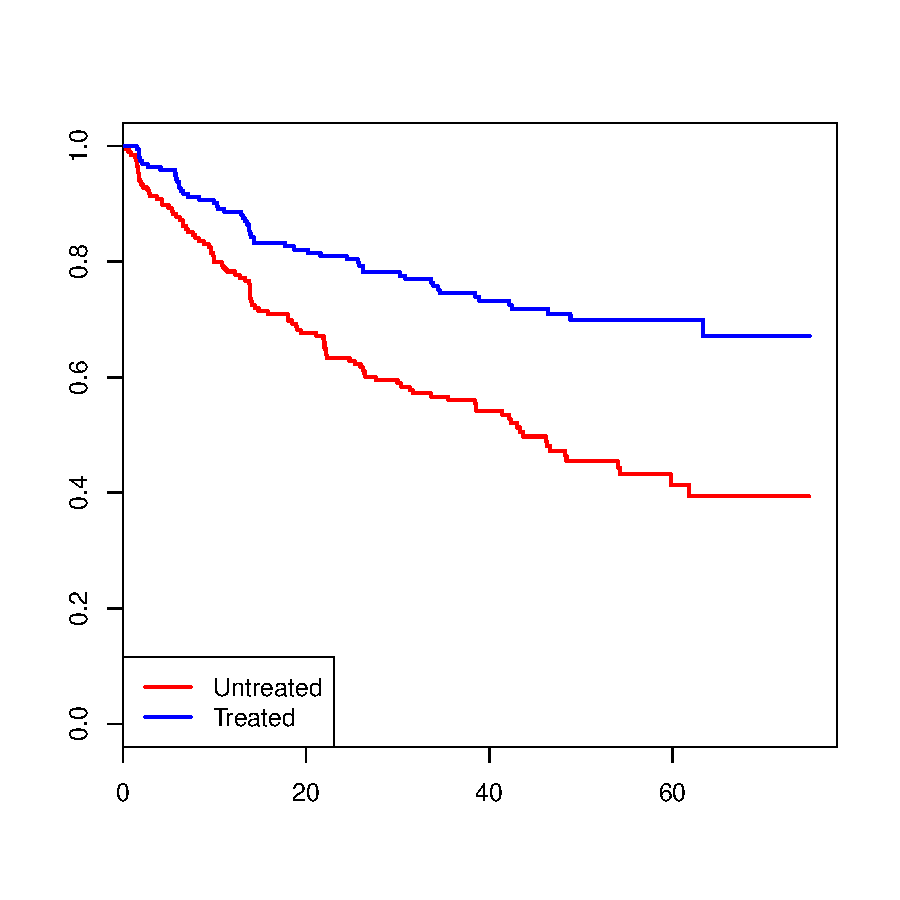
\includegraphics{StatisticalBackground-003}

Visually examining these curves, we can see right away that untreated eyes are experiencing diabetic retinopathy at a much higher rate than treated eyes. Note that these curves do not go below 0.6 and 0.3. This is because a large percentage of the subjects never experienced diabetic retinopathy during the course of the study, so one cannot obtain non-parametric estimates of the tails from the data alone. 
    
    \subsubsection{NPMLE}
  
  Just as the Kaplan Meier curves are a generalization of the EDF that allows for right censoring, the non-parametric maximum likelihood estimator (NPMLE) is a generalization of the Kaplan Meier curves that allow for general interval censoring. In the case that each event time is known to be in the closed interval $[L_i, R_i]$, the estimator can be written as
  
\[
  \hat S(t) = \arg \max_S 
  \displaystyle
  \sum_{i = 1}^n \log(S(L_i^{-}) - S(R_i))
\]
\[
  S(t) \in [0,1]
\]
\[
  S \text{ decreasing}
\]

  It can be shown that with only right censored data, the NPMLE will result in the Kaplan Meier estimator. In the general case, the NPMLE is not in closed form and must be solved for iteratively. 

  The NPMLE assigns probability mass only to \emph{Turnbull intervals}. A Turnbull interval is an interval $[L_i, R_j]$ made up of the left and right side of (potentially different) observation intervals such that no other end points lie inbetween. How the probability is assigned within these intervals does not affect the likelihood function, so the NPMLE is defined only up to an interval (although with ties in the data, these intervals can be of length 0). This is sometimes referred to as \emph{representational non-uniqueness}. To demonstrate this, we borrow the \texttt{bcos} from the \texttt{interval} package. 
  
\begin{Schunk}
\begin{Sinput}
> library(interval)
> data(bcos)
> # Fit the NPMLE for each treatment group
> npmle_fit <- ic_np(cbind(left, right) ~ treatment,
+              data = bcos)
> plot(npmle_fit)
\end{Sinput}
\end{Schunk}
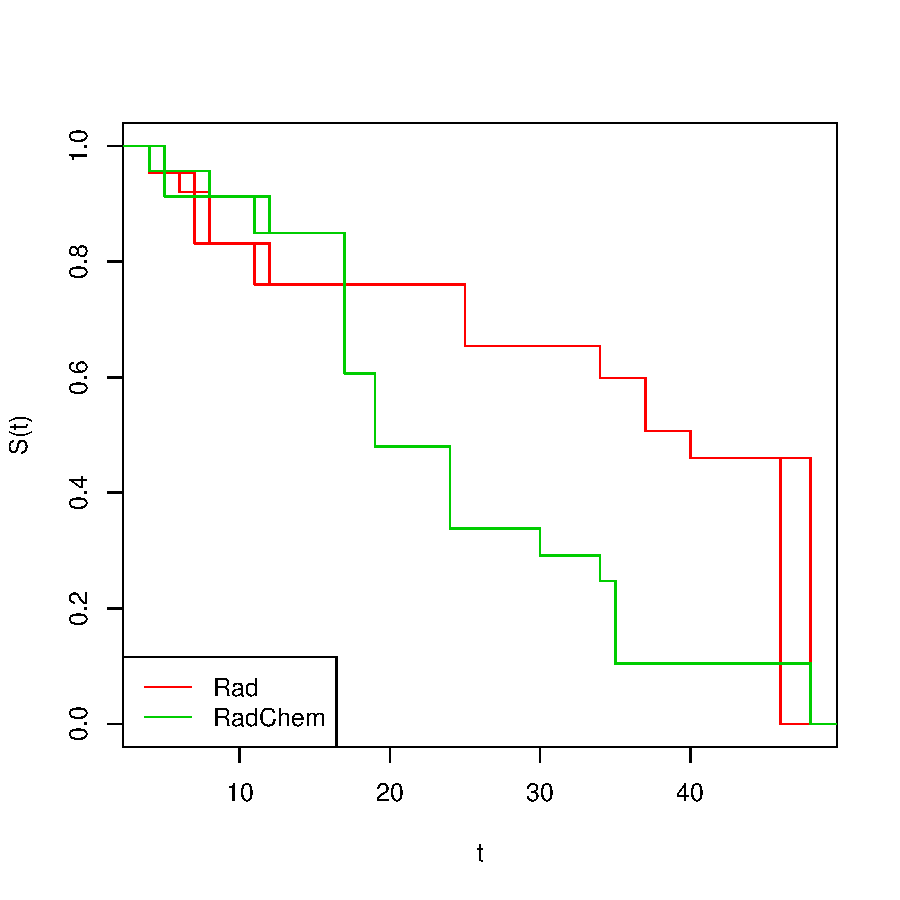
\includegraphics{StatisticalBackground-004}

  Note that for some sections of each estimated survival curve, the estimated survival probability is given up to an interval, rather than a single point estimate. This is a realization of representational non-uniqueness. 
  
  For the remainder of this work, we will use the \texttt{IR\_diabetes} data set for demonstrational purposes. Below is the plotted NPMLE. 
  
\begin{Schunk}
\begin{Sinput}
> npmle_fit <- ic_np(cbind(left, right) ~ gender, 
+                    data = IR_diabetes)
> plot(npmle_fit, col = c('purple', 'orange') )
\end{Sinput}
\end{Schunk}
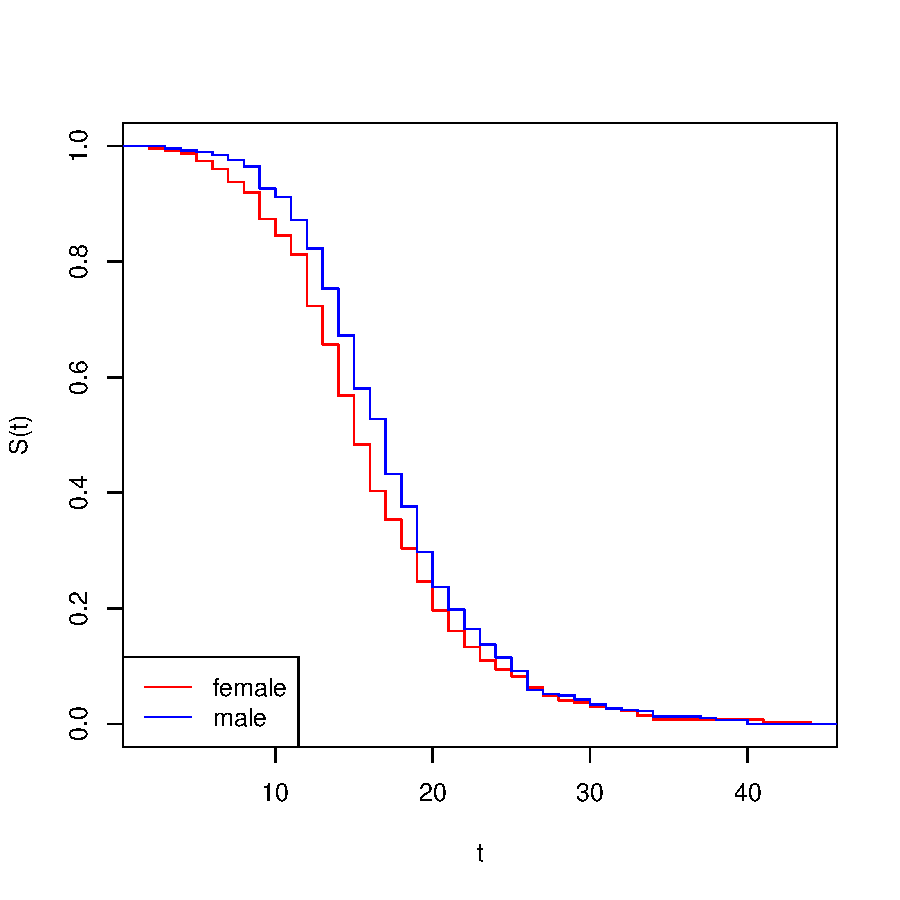
\includegraphics{StatisticalBackground-005}

We note that visually, there appears to be no issue with representational non-uniqueness in this example. This is due to the many ties in the data, which collapse the Turnbull intervals down to a single point for any given $t$. 

  \subsubsection{Parametric Models}

  Using the likelihood functions presented in \ref{sec:llk}, standard fully parametric maximum likelihood (MLE) or Bayesian models can be fit for censored data. Commonly used parametric families include the exponential distribution, Weibull, gamma, log-normal and log-logisitic to name a few. Note that for all these models, $S(0) = 1$, a standard assumption in survival analysis. 
  
  In partice, the single parameter exponential distribution 

  \subsection{Regression models}
  
  Generalized linear models (GLM's) have the relation that 
  
  \[
  E[y_i | x_i, \beta] = g(x_i \beta)
  \]
  
  where $g$ is the link function connecting the linear predictor ($x_i \beta$) to the conditional mean of $y_i$. Traditional survival regression models are linear models, similar to GLM's, but the effect of the covariates can typically be most succinctly  described as an effect on various baseline survival functions rather than the expected value. As such, survival regression models will typically be defined so that they can be written as 
  
  \[
  S(t | x, \beta) = g(S_o(t), x \beta ) 
  \]
  
  where $S$ represents the survival function conditional on the covariates and regression parameters and $S_o$ represents the baseline survival distribution, i.e. the survival distribution for a subject with all 0 covariates. 
  
    \subsubsection{Proportional hazards}
    
    One of the most popular regression models is the proportional hazards model. The model can be defined as
    
    \[
    h(t_i|x_i, \beta) = h_o(t_i) e^{x_i \beta}
    \]
    
    where $h(t|x_i, \beta)$ is the hazard for subject $i$ conditional on covariates $x_i$ and $h_o(t)$ is a baseline hazard rate, \emph{i.e.} the hazard rate for a subject with covariates all equal to 0. In other words, for a subject with covariates $x_i$, their current hazard is $e^{x_i \beta}$ times higher than a baseline subject at any given time.
    
    Note that the relation between the hazards rates is constant as a function of time enforcing the \emph{proportional-hazards} assumption, which should be inspected.  For example, consider a hypothetical experiement with two groups of cancer patients, one treated with chemotherapy, one not receiving treatment. Chemotherapy is an extremely damaging treatment, so shortly after treatment, the chemotherapy group will have higher hazards than the untreated group. However, once the treated group recovers from the chemotherapy, they are at much lower risk than the untreated group. 
    
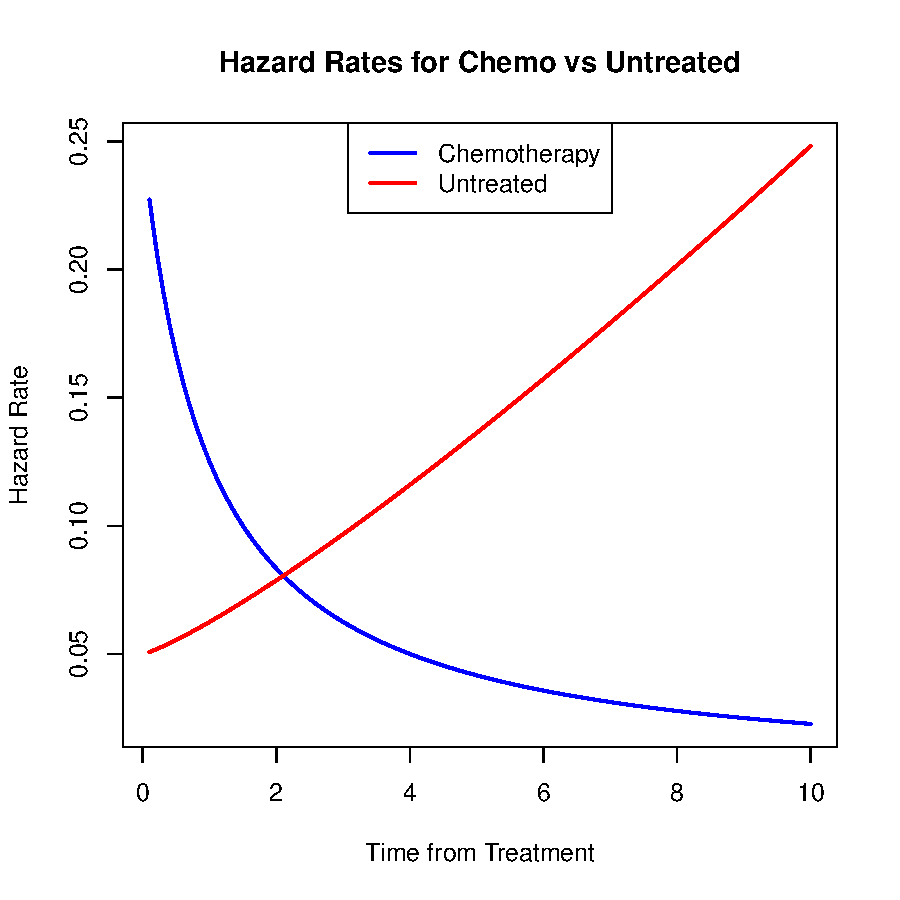
\includegraphics{StatisticalBackground-006}
    
    A typical rule of thumb for assessing proportional hazards is that if the estimated survival curves cross, the hazards are likely non-proportional\footnote{An exception to the crossing survival curves rule is that crossing of the estimated extreme tails is less worrisome, as estimates of the extreme tails are typically very noisy.}. It's worth noting that crossing survival curves is a much stronger condition than non-proportional hazards. As such, crossing survival curves should be seen as evidence of \emph{very strong} violations of the proportional hazards assumption. Other methods for will be discussed shortly. 
    
    Using the relation 
    $S(t) = e^{\int_{-\infty}^t -h(x) dx }$,
    we calculate the survival curves from the hazard curves in the chemotherapy treatment example. We see that the survival curves do in fact cross for the two groups. 
    
    
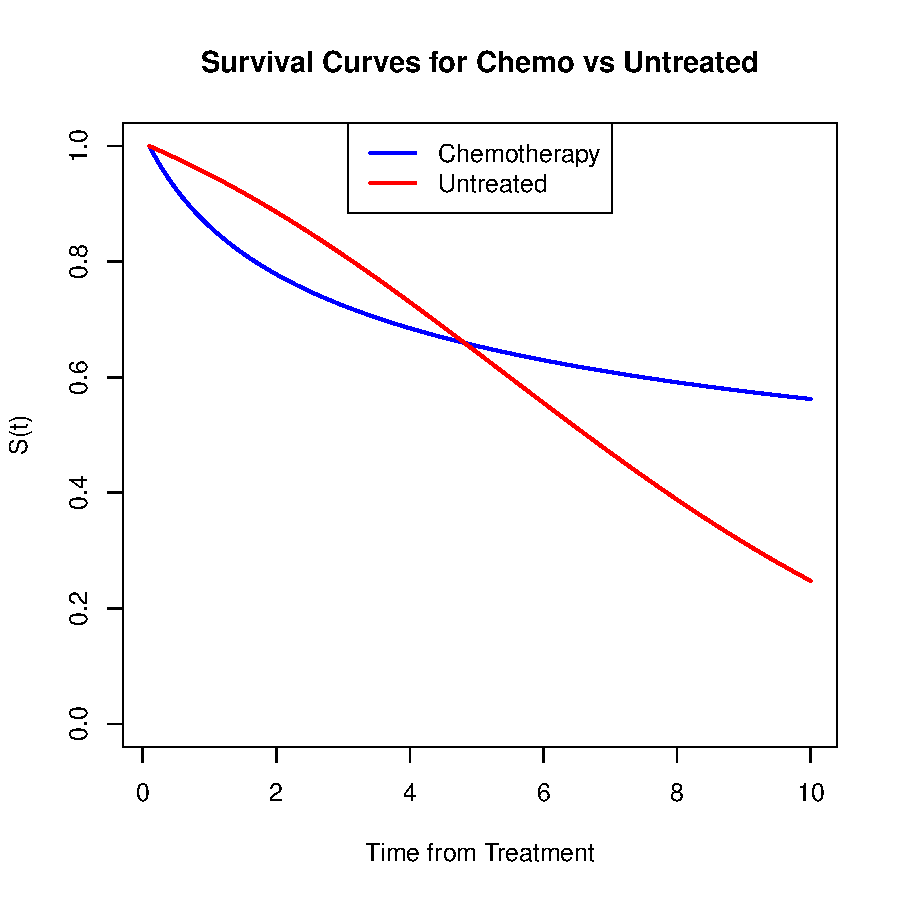
\includegraphics{StatisticalBackground-007}

  With a little bit of algebra, it can be shown that the proportional hazards assumption is equivalent to 
  
\[
  S(t| x, \beta) = S_o(t)^{e^{x \beta}}
\].

    \subsubsection{Accelerated failure time}
   
   The accelerated failure time (AFT) model is built on the relation
   
   \[
   S(t | x, \beta) = S_o(t e^{-x \beta})
   \].

    In otherwords, subjects with $x = 1$ experience events $e^{-\beta}$ times faster than subjects with $x = 0$. One advantage of the AFT model is the ease of interpretation; it is very common for casual users of survival analysis to interpret a Cox-PH model as an AFT model, i.e. it is a common mistake to state that doubling the hazard implies events occur twice as fast. 
    
    If the baseline survival distribution $S_o$ is a Weibull distribution, then the AFT model is equivalent to the proportional hazards model, up to a linear transformation of the regression parameters. In such a case, it is recommended to use the AFT parameterization due to easier interpretation of regression coefficients. It does not hold that these models are generally equivalent, however. 
    
    \subsubsection{Proportional odds}
  
  The proportional odds model is built off the following relation:
  
  \[
  \frac{S(t|x, \beta)}{1-S(t | x, \beta)} = e^{x \beta} \frac{S_o(t)}{1 - S_o(t)}
  \].

  In otherwords, the odds of survival at any given time is $e^{\beta}$ times higher for a subject with a one unit higher value of $x$. Interestingly, with the special case of current status data, it can be shown that fitting a proportional odds model is equivalent to using logistic regression with $\log(t)$ as a predictor. 
  

\end{document}
